%%%%%%%%%%%%%%%%%%%%%%%%%%%%%%%%%%%%%%%%%%%%%%%%%%%%%%%%%%%%%
%% HEADER
%%%%%%%%%%%%%%%%%%%%%%%%%%%%%%%%%%%%%%%%%%%%%%%%%%%%%%%%%%%%%
\documentclass[a4paper,twoside,11pt]{article}

%% Language %%%%%%%%%%%%%%%%%%%%%%%%%%%%%%%%%%%%%%%%%%%%%%%%%
\usepackage[T1]{fontenc}

%\usepackage[ansinew]{inputenc}
\usepackage[utf8]{inputenc}	%supports Umlaute
%\usepackage{german, ngerman}
\usepackage{color}

\usepackage{lmodern} %Type1-font for non-english texts and characters

%% Packages for Graphics & Figures %%%%%%%%%%%%%%%%%%%%%%%%%%
\usepackage{graphicx} %%For loading graphic files
\usepackage{multicol}

%% Math Packages %%%%%%%%%%%%%%%%%%%%%%%%%%%%%%%%%%%%%%%%%%%%
\usepackage{amsmath}
\usepackage{amsthm}
\usepackage{amsfonts}
\usepackage{amssymb}

%% Line Spacing %%%%%%%%%%%%%%%%%%%%%%%%%%%%%%%%%%%%%%%%%%%%%
\usepackage[parfill]{parskip}    % Activate to begin paragraphs with an empty line rather than an indent

%% Other Packages %%%%%%%%%%%%%%%%%%%%%%%%%%%%%%%%%%%%%%%%%%%
\usepackage{a4wide} %%Smaller margins = more text per page.
\usepackage{fancyhdr} %%Fancy headings

%%%%%%%%%%%%%%%%%%%%%%%%%%%%%%%%%%%%%%%%%%%%%%%%%%%%%%%%%%%%%
%% DOCUMENT
%%%%%%%%%%%%%%%%%%%%%%%%%%%%%%%%%%%%%%%%%%%%%%%%%%%%%%%%%%%%%
\begin{document}

\pagestyle{fancyplain}

%% Title Page %%%%%%%%%%%%%%%%%%%%%%%%%%%%%%%%%%%%%%%%%%%%%%%
\title{Parallel Programming Assignment \#3} 
\author{Marcel Karsten -- 343619,\\ Patrick Lorenz -- 341922,\\ Richard Klemm -- 343635 }
\date{Due: Thursday, 7th June 2012} %%If commented, the current date is used.
\maketitle

%% Header on top of every page (yes, also on the title page!)
\rhead{Parallel Programming - TU Berlin, SS/12}
\lhead{}
\renewcommand{\headrulewidth}{0px}


%%%%%%%%%%%%%%%%%%%%%%%%%%%%%%%%%%%%%%%%%%%%%%%%%%%%%%%%%%%%%

\section{Exercise 1 - Parallel Algorithm Design}

\textbf{(a) Mapping to a regular scan}

$x = f(\text{a}_i,\text{f}_i) = \begin{cases} x = \text{a}_i & \text{if } \text{f}_i = 1 \\
								x = -\text{b}_{i-1} + \text{a}_i & \text{if } \text{f}_i = 0 \\
\end{cases}$

$x = \text{a}_i  - ( \text{b}_{i-1} * \text{f}_i)$

not associative?!

%\begin{cases}  x = \text{a}_i & \text{if } \text{f}_i = 0 \vee i = 0\\
%								x = \text{a}_i  + \text{b}_{i-1}& \text{if } \text{f}_i = 1	  %\end{cases}$
%\sum\limits_{n=1}^{\text{f}_{i-n} = 1}\text{a}_{i-n}


\textbf{(b) Parallel Scan}

\begin{figure}[hbtp]
\centering
\label{fig:para_algo}
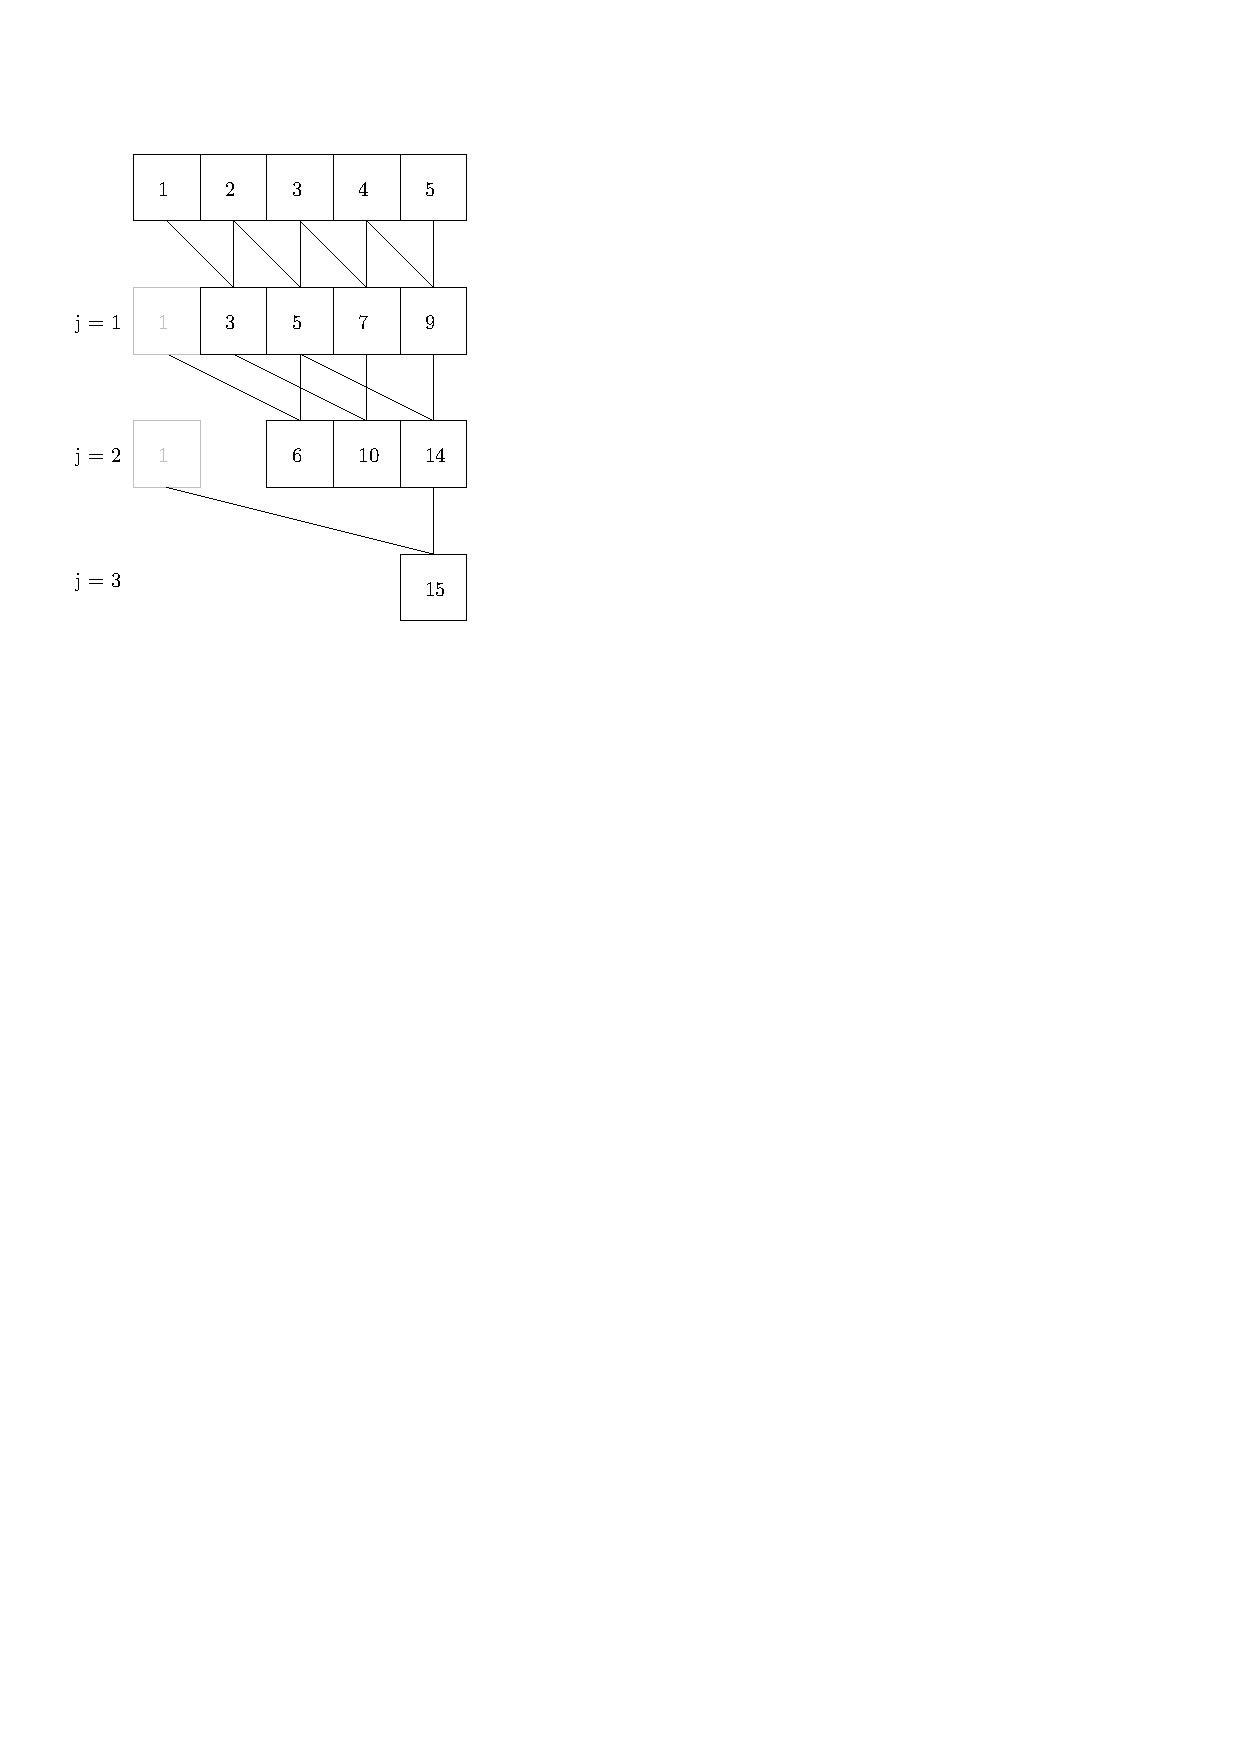
\includegraphics[scale=1]{algo}
\caption{Parallel Scan}
\end{figure}

\begin{tabular}{|p{3cm}|p{6cm}|l|}
\hline
Property&Parallel Scan& Sequential Scan\\
\hline
\hline
\#Opertaions& $\sum\limits_{j=1}^{\log_2n}(n-2^j+1)$& $n-1$\\
\hline

Execution time depending on n/p & $p \ge n -1 : \log_2n$ \newline ca.  $p < n -1 : \log_2n * n/p$& $n-1$\\
\hline

\end{tabular}

While the parallel scan is much faster than the sequential scan, it has  a couple of drawbacks. Most noticeably it does not accept all input lengths.

Analysis of the algorithm is ignoring communication overhead, as it is assumed that all parallel operations can be executed simultaneously.



\textbf{(c) Handling many elements}




\end{document}
